\documentclass[12pt]{article}

\usepackage[margin=1in]{geometry}
\usepackage{xcolor}
\usepackage{graphicx}
\usepackage{url}
\usepackage{hyperref}

\newcommand\TODO[1]{\textcolor{red}{#1}}
\newcommand\todo[1]{\textcolor{red}{#1}}

\begin{document}
\title{Fine-grained Access for Securing NFC:  Distributed Key Association}
\author{Max Feldman \and Stephanie Rogers \and Richard Xia}
\maketitle

\section{Abstract}
Near Field Communication (NFC) is a form of contactless communication that allows devices to transfer data over radio; it is similar to RFID, but with a much smaller range of use.
NFC has existed for some time, but its implementation in Android phones, along with an API for developers, has only recently gained popularity.
Upon scanning an NFC tag, Android will automatically run the application that has been associated with the type of data on that tag, sometimes without user interaction or approval.
The Android NFC API offers application developers a new, more powerful means to access NFC capabilities in mobile devices, but this introduces an increased attack space and additional potential for vulnerability.
Android provides access to an NFC Data Exchange Format (NDEF) API, but does not offer any of the various security measures that have been proposed.

We examine the growing space of NFC applications offered for Android, and provide a cursory categorization of the functionality and general security practices of these applications.
Alarmingly, several applications implement features such as SMS messaging or calling given phone numbers, or accessing arbitrary URLs, which are provided by an NFC tag without even prompting the user.
We attempt to address the issue of resource access on behalf of external data, in the context of NFC.
We discuss known issues and vulnerabilities with NDEF security, and how our proposal mitigates some of these concerns.
We also keep in mind the importance of usability, especially in applications that must perform quickly and smoothly--as is the case with NFC applications. Finally, we present the description of a user study that can effectively evaluate the tradeoffs between secure access control and usability.

\TODO{\section{Introduction}}
1-2 page version of paper

\section{Background}
Near Field Communication (NFC) is an emerging technology for wireless communication that allows NFC-enabled devices to transfer small amounts of data at a close proximity, usually no more than a few centimeters.
At the most basic level, NFC specifies a set of protocols for this wireless communication based off of the radio-frequency identification (RFID) standards.
NFC offers current and predicted functionality of contactless transactions, data exchange and an alternative to traditional contactless technologies such as RFID and QR codes.
NFC-enabled devices can use the protocol in two modes: active and passive.
In passive mode, there is a device actively generating a radio frequency (RF) field that initiates contact to the passive NFC tag.
An NFC tag is a passive device that stores data for NFC transmission.
There are several types of NFC tags, but in general they are a means of persistent storage for NFC data.
Depending on the type of tag, the data can be overwritten or modified, or require authentication from a reader before transmitting its data.
In this case, the device can read or write information stored on NFC tags and cards without the passive targets needing any power source.
Active devices are also able to emulate NFC tags by transmitting NFC data.
For the purpose of discussion within this paper, we use ``tag'' to refer to either a physical tag, or a device which is emulating a tag, as their functionality is the same within the context of our exploration.
Additionally, NFC phones have the ability to communicate with other NFC-enabled mobile phones to transfer data peer-to-peer in active mode.
In this case both devices are generating their own RF fields.

\subsection{Android NFC}

The Android system sends and receives NFC data in the form of NFC Data Exchange Format (NDEF) messages.
These messages, which are stored in the NFC tag, act as a container for one or more NDEF records which are further broken up into a header and a payload, which contain typed data such as MIME-type media, a URI or a custom application payload.

\begin{figure}[h!]
\begin{minipage}{\textwidth}
	\centering
		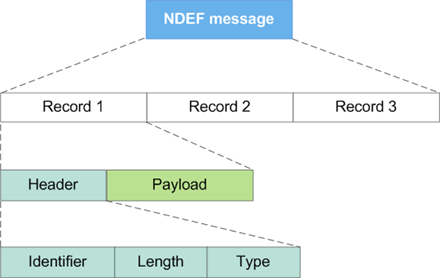
\includegraphics[width=0.5\textwidth]{NDEF_Format.png}
	\caption[Caption for LOF]%
		{NDEF Message Format\footnote{\url{http://www.developer.nokia.com/Community/Wiki/Understanding_NFC_Data_Exchange_Format_(NDEF)_messages}}}

\end{minipage} 
\end{figure}

Specifically, the Android system offers the ability to read and write NFC tags for passive mode, and beam NDEF messages from one device to another with Android Beam.\footnote{\url{http://developer.android.com/guide/topics/connectivity/nfc/nfc.html}} for active mode. 

\subsection{Android Intents}
The core components of an Android application are activated through messages called intents.\footnote{\url{http://developer.android.com/guide/components/intents-filters.html}}
Intents are used for inter-application and intra-application communication by sending messages with relevant information about operations to be performed to various applications.  

When NFC is enabled and the screen is unlocked, Android devices will always be searching for input from an NFC tag or device. 
When the device discovers an NFC tag, the Android OS creates an intent that is dispatched to an application that has registered for it.
This information is processed by Android's special tag dispatch system to determine which activity to launch.
In the case that more than one application can handle the type of data contained in the tag, the phone will open a prompt for the user to choose among the several applications; however, if there is only one application, the phone will automatically launch this application and process the tag.
NFC input can force Android phones (with certain settings) to parse images, videos, contacts, and office documents, call or text arbitrary phone numbers, establish Bluetooth connections, and open web pages via the browser, all without user interaction.  

\subsection{Android Permission System}
Android applications run in a sandbox that allows areas of the system to be isolated and thus limit access to the security-related parts of the Android API.
However, access to these resources can be granted to an application if the developer requests the appropriate permissions in the application's manifest.
Android developers are expected to use least-privilege with their permission requests: limit the permissions requested to only those that are absolutely necessary for the function of their applications. 
% not sure we need to \TODO{Relate this back to NFC.}

\section{Threat Model}
While NFC is still an emerging technology, there are several vulnerabilities that can afflict applications.
In our work, we address three of these: malicious NFC tags, more generally, fraudulent data inputs, and threats on user privacy.
\subsection{Malicious Tags}
We define a malicious NFC tag as an NFC tag that contains data that would cause a user to act on data which they did not expect.
If the attacker has the ability to automatically have the phone call a specified number, then a tolled number could easily be inserted and thus result in a monetary loss on the part of the user. 
An example of an application that does this is Samsung's Tectile\footnote{\url{http://www.samsung.com/us/microsite/tectile}} application which, when scanning a tag with a phone number and directions to call this number, will do so without any further user prompts.
For example, an attacker could replace the tag on a poster advertising a local event with a new tag, containing a paid phone number.
When a user swipes the tag to view the event's website, their phone will place a call and their account will be billed.

\subsection{Privacy Concerns}
Several NFC applications have the possibility of writing information to an NFC tag.
This means that users have the ability to write anything they want to their own tags.
It may be beneficial for some users to use these tag writing applications to write sensitive or critical information to tags they keep in specific locations.
However, if encryption is not used, an attacker who can gain access to these tags will have unfettered access to their information.
NFC is also used as a means of initiating connections on higher-bandwidth media (eg. Bluetooth), but if this connection handover is interfered with then an attacker may be able to listen in on the new connection.

\subsection{Unaddressed Threats}
There are several other threats to consider, which we mention here, but are outside the scope of our project.
In ``Securing Near Field Communication'' \cite{kortvedt2009}, Kortvedt, proves that it is possible to eavesdrop on NFC communication using simple equipment and methods.
Since the NFC communication protocol does not offer any security or encryption itself, it is up to the developer to implement or use encryption to secure the data within the application's code. 

We also omit discussion of relay, replay, and denial of service attacks.
A relay attack exploits the assumption that two devices engaged in an NFC transaction are actually adjacent (by placing a proxy in between the two devices).
This is a serious potential exploit which must be defended against by any security-conscious application (as it may allow for arbitrary credit card purchases, for example).

\subsection{Relevant NFC Technology and Security}
It is important to address the related technology to NFC and some of the protocols implemented and proposed that already attempt to deal with the above NFC issues. 

MiFare, FeliCa and AFAICT are all contactless smart cards that can acts as tags for NFC devices and each offer different security features. MiFare is hardware that allows the locking of data once it is written on the tag and allows symmetric mutual authentication of users and write protection to defend against reading and writing of the tag. FeliCa provides authenticaton and write protection as well. The purposes of MiFare and FeliCa are to provide privacy to the user; however, the focus is to authenticate users rather than tags. AFAICT has the ability to lock the data to make it not overwritable, but does not provide authentication. As each type of tag only offers a subset of the security measures that are possible, it is left to the developer to provide some sort of security scheme or use cryptography to provide privacy. 

In addition to the security that various NFC technologies have provided, there has been much insight into the vulnerabilities of NFC at the network-level. 
One major foray into such analysis was presented by Charlie Miller at BlackHat 2012\cite{miller2012}.
Miller employs fuzz testing to show that carefully crafted NFC payloads can do much more than just crash a device---in some cases phones can be forced to parse arbitrary data or open web pages without user interaction.
Miller's work provides a wide analysis of the NFC attack surface, but our research will seek to provide much more depth in the exploration of application-level vulnerabilities.

RFID, a precursor to and superset of NFC, has also raised several security issues in the past.
Though RFID is a much older technology, it is remains relevant as both the foundation for NFC, and as a technology which is still employed in various applications (most prominently touch-activated credit cards).
Several issues involved in early generation deployments of RFID credit cards were discovered through the successful implementation of various attacks on three major RFID enabled credit cards (including attacks which access private information or enable arbitrary purchases by the attacker)\cite{heydtbenjamin2007} .
%Such attacks remain important considerations due to the growing prominence of smartphone payment applications  (such as Google Wallet), so we keep all of these vulnerabilities in mind as we explore NFC security vulnerabilities.

%Haselsteiner et al\cite{haselsteiner2006} discuss general security issues with NFC (beyond the scope of just mobile phones).
Further analysis at the application-level has showed threats of eavesdropping, data corruption, data modification, data insertion, relay attacks\cite{francis2012}, and man-in-the-middle attacks (though MITM is dismissed as practically impossible).
One solution which involves setting up a secure channel between devices in order to prevent such attacks\cite{haselsteiner2006} is presented but not implemented. As our focus is restricted to Android devices, we have the ability to recommend and implement Android-specific solutions to some of the above attacks. 
%Francis et al.\cite{francis2012} discuss the potential for relay attacks on NFC transactions, and implement a software version of this attack which can be used on an NFC-enabled device.
%The paper suggests several potential counters to such attacks; our analysis examines how popular applications employ relay-attack countermeasures, and to what degree they are effective.
%\textbf{Random shit}
%Analysis of smartphone applications in general (though we restrict our focus to Android devices, as iPhones do not yet offer NFC) is a much more thoroughly explored field, and several projects provide valuable insight into application testing.
%While RFID technology and Android application analysis have both been explored, there has been very limited exploration of Android-specific NFC applications, and their potential vulnerabilities.
%We leverage this previous exploration to provide large-scale analysis of NFC applications, vulnerabilities, and coding practices, as well as to recommend best practices for preventing NFC attacks.

\section{Related Work}
%Close range radio wave communication has existed for some time, but the application of NFC in mobile phones is a recent development and still growing in popularity.
The NFC Forum\footnote{\url{http://www.nfc-forum.org/}}, which publishes NFC standards\footnote{\url{http://www.nfc-forum.org/specs/spec_list/}} and best practices, was only formed in 2004.
The relative youth of this field has resulted in many aspects remaining largely unexplored.
In this section we present relevant past work in the area of NFC security, as well as mobile phone application security in general.

\textbf{Pre-shared keys.}
One approach for authenticating tags is to share keys between tag readers and tag writers.
Kortvedt \cite{kortvedt2009} proposes a general framework for providing one-way and mutual authentication over NFC, but requires the use of pre-shared keys.
He suggests using a centralized key authority associated with mobile carriers such as Over-The-Air (OTA) programming or SMS for distributing keys.
We believe is impractical and inappropriate for all types of applications given that tag authors may be distinct from application authors and may wish to distribute keys.
There is also no notion of trust, as a user must trust that the key being shared is legitimate.
We instead seek to provide a decentralized mechanism for trusting and granting trust to a user-defined set of NFC tag authors.

\textbf{Signatures and Certificates.}
The NFC Signature Record Type Definition (RTD), which can be used to sign NDEF records, was standardized to deal with threats caused by malicious tags including spoofing, phishing and denial of service.
Using signatures on a tag causes a performance and space penalty, which are important since NFC tag readers are mobile devices and NFC tags themselves have very limited storage space \cite{kilas2009}.
The standard now focuses on being able to authenticate the source of data through a certificate authority which distributes and validates public keys \cite{rosati2011}.
However, vulnerabilities arise with these signature records when mixing signed and unsigned records in a single NDEF message \cite{roland2010,roland2011}.
We propose a way for users to authorize keys based on the data type and application, which are enough to determine a fixed behavior (e.g. calling a phone number from a tag or opening a URL stored on a tag).


\section{Proposed Solution}
We propose a system of controlling the access that NFC inputs are granted by the Android OS.
This access control system aims to provide a simple and usable means for phone users to grant access to certain capabilities to trusted tag authors.
A capability in this case refers to the ability to access a system resource, such as to call a phone or open a URL.
We differentiate this from a permission (which individual applications must request), in that it is more restrictive, and specific to a tag author (as identified by their public key).
This system uses per-application access control to specify approved, unapproved, and unencountered access-requestors.
We specify the goals and non-goals of our system and then outline the approach in detail, as well as discuss our implementation.
\subsection{Goals}
The principal goal of this system is to allow users to link their trust with their access policies.
The user's trust should define the access granted to external entities.
If a user trusts a particular tag author to provide non-malicious URLs, then the user can grant that tag author approval for all URLs in the context of that application.
This system must be fast and unobtrusive, so that the short duration of an NFC interaction is not impeded.
The system must also be simple, for both users and application developers.
Users should be able to understand what access policies they choose to grant, and administer these policies with ease.
This includes granting additional access and revoking existing access.
\subsection{Non-goals}
We do not seek to provide trust mechanisms for users.
At best, we wish to leverage existing trust mechanisms (such as certificates included in Signed NDEF records), but present the information regarding the identity of an author in an easy-to-read format.
If the signer of a tag is identified in a certificate chain, then it is important to present the user with that identity so that the user can make an informed decision regarding access control.
We do not seek to offer integrity or authentication.
These are both goals of the NDEF Signature RTD, and as such we leverage these properties but do not duplicate the effort of providing them.
This system does not offer an alternative to the certificate scheme support by the NDEF Signature RTD.
\subsection{Approach}
In order to provide fine-grained access control, each application maintains its own access control list.
An entry in this list consists of the TNF of the NDEF record, the Type of the NDEF record, and the public key extracted from the signature which applies to that record.
This system is intended to be an OS library which allows developers to grant, revoke, and verify access within the context of their application.
When a tag is read, its data will be marshalled to the appropriate application, if that application is not already running.
\begin{figure}[h!]
\begin{minipage}{\textwidth}
	\centering
		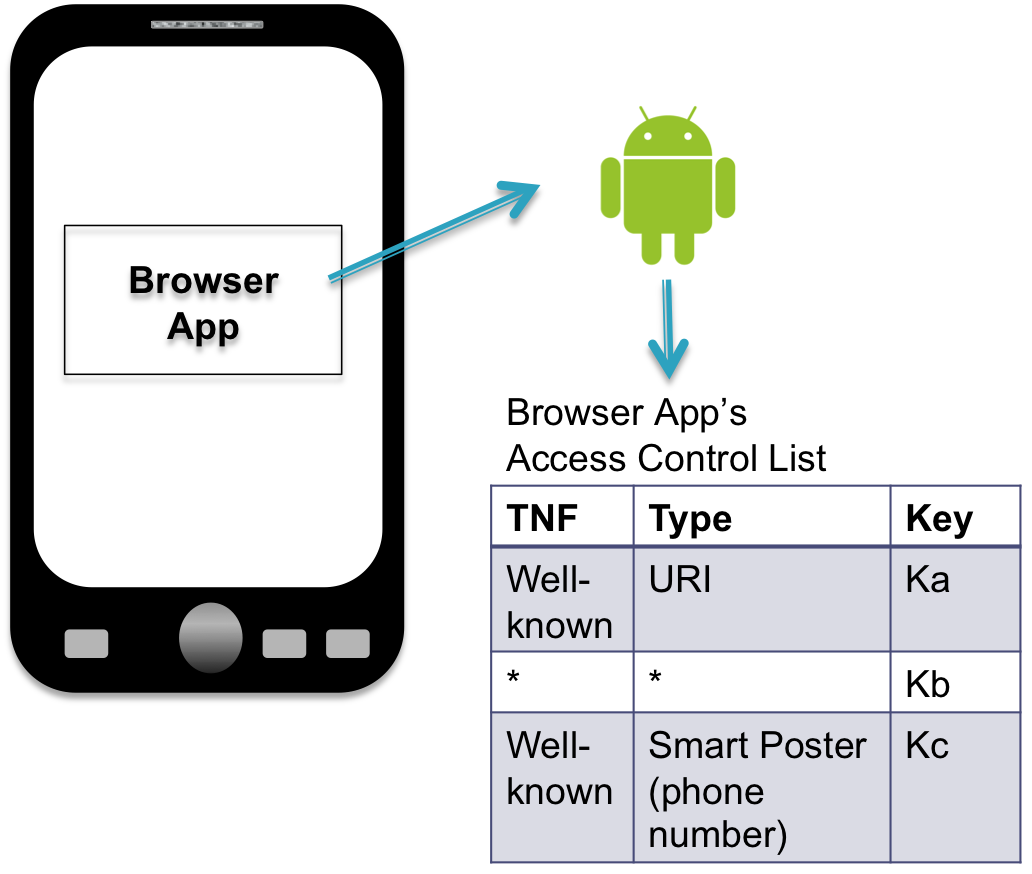
\includegraphics[width=0.5\textwidth]{ACL_image.png}
	\caption[Caption for LOF]%
    {An example of an application utilizing its access control list. The Browser application has three entries in its access control list. Ka is a key which is granted access for URI-type tags. Kb is granted access for all tag types. Kc is granted access for phone numbers, found in a Smart Poster tag. The Browser application interfaces with this access control list via the OS.}

\end{minipage} 
\end{figure}
\subsubsection{Verifying Access}
Before an application acts on NDEF input data, it verifies that the NDEF record's type and public key (from the associated signature record) exist in the access control list.
The OS provides a method call which allows the application developer to easily check whether this content author has been approved.
The application developer is encouraged to rely on well-known types, but types examined for access control can ultimately be specified by the developers.
It is important to allow a degree of developer control over the types examined, as the logic of the application may leverage types in ways which the OS cannot predict.
This content author can either be approved for a specific type (TNF and Type field), or for all types.
For example, an author with public key Ka may have a record [001:55:Ka], indicating that their key is trusted for all URI inputs within the context of that application.
Another author with public key Kb may have a record [*:*:Kb], indicating that they will always be granted access by this application.
If the lookup of [TNF:TYPE:Key] returns true, then the data's provider has been granted access and operation proceeds uninterrupted.
If the lookup fails, then a user will be prompted to either allow the operation to proceed once (ie. without granting permanent access), grant permanent access, or deny access and abort the operation.
\subsubsection{Granting Access}
If a user elects to grant access upon receipt of NDEF data, then they will be given the option of granting the tag author permanent access for that NDEF type (TNF and Type fields, or an application-developer-specified type), or for all types (a wildcard match on the TNF and Type fields).
The OS will then attempt to deliver the most readable identifier of the public key which the user is about to approve.
In most cases, extracting the identifying information from the certificate will be sufficient to present the user with a concise identity of the content author.
The user then chooses the type of access they wish to grant to that public key, and this access choice is written to the access control list for that application.
\subsubsection{Revoking Access}
Users will be provided an interface to the access control lists for their applications by the OS.
Through this interface, the user can view all authors to which they have granted access (including the human-readable name associated with the public key).
The user can then choose to revoke access to an author by removing associated entries of that author in relevant lists.
The user can also remove only one access grant to an author, if they so choose.
Revocation should additionally support certificate revocation lists; if a tag with a revoked certificate is encountered, that revocation should propagate to the access control list.
Additionally, if a certificate has been found which is outside its validity period, the access associated with that identity should be revoked.


\subsection{Alternatives}
One access control method we considered was requiring approval when data was handed over to another process, as opposed to approval upon reading the data.
For example, in this scheme if an NFC tag contains a phone number, the user would be prompted to approve the outgoing phone call.
A method such as this could offer persistent approval, as our proposal offers.
After a user approves a phone number to make calls, any further calls would not require further user approval.
We avoid this approach, however, as we feel it is not generalizable in a usable way.
Opening arbitrary URLs presents a significant attack vector in NFC tags.
However, usability of such a scheme decreases drastically if a user must approve every new URL encountered on NFC tags.
We believe that the number of tag authors will be lower than the number of resources a user encounters on NFC tags, and as such, author-based access control provides a more generalizable (and still usable) approach.

We also considered the merits of allowing access sharing between applications.
The principal benefit of such a system is that there would no longer be duplicate access granting if a user wishes to trust a tag author within the context of multiple applications.
While this would easily be possible, it raises two major concerns.
First, shared access control would open the possibility for malicious applications to inject additional trust for authors who may otherwise be untrusted.
An additional permission for read and write access to the shared access control list would need to be introduced in order to better manage which applications can alter this control list.
Second, there are cases in which sharing access would result in a loss of security.
For example, if one application with limited permissions added a tag author, \textit{A}, as a trusted author for all tag types, this access could be shared with other applications.
If another application with more permissions (such as \texttt{CALL\_PHONE}) saw \textit{A} as having access to all tag types, \textit{A}'s tags would then be able to place phone calls.
There are means to mitigate this threat, but the management becomes significantly more complicated, and simplicity is a necessary facet of our proposal.

\section{Implementation}
We begin implementing our access control system as an Android library that Android developers can include and access in their projects.
Unfortunately, Android does not yet support the NDEF Signature RTD, so much of our work involved working around this.
We provide an API as a proof-of-concept for the proposed access control scheme, through which developers can add, verify, and revoke access.
Our current implementation simply creates a makeshift signature record consisting of a digital signature (created by DSA) appended to the public key used for the signature.
This emulates the PKI infrastructure provided by certificates, but in a simpler manner, as the focus of our proof-of-concept is the access control itself.
We present this implementation as a proof-of-concept; ideally, such additions to the Android NFC stack would be implemented at OS-level.
There are several advantages to kernel modifications, which are discussed below.

\subsection{Access Management}
Users need to be able to grant and revoke access to resources, either manually, or in the context of a tag reader application.
For our API, we use Android's \texttt{SharedPreferences}, which provides persistent key-value storage.
Our current implementation provides a unique instance of this access control list (ACL) to an individual application.
A given application can only access and modify its own access grants (aside from the OS interface provided to the user).
In order to provide an OS library, as well as key management through OS utilities, the access control system must be implemented at OS-level.
The Android Library we implement allows developers to effectively leverage access control, but more features and simplicity would be achieved by integration into Android itself.

\subsection{Recommendations for Kernel Implementation}
We have presented the advantages of an OS implementation of this system.
No additional permissions would be required of this implementation, as applications can only modify their own access control lists.
An application would therefore not be able to falsely influence the access granted on behalf of other applications.
An OS implementation allows for a consolidated and secure means of providing developers with a library for access control, and users with a centralized means of viewing and managing the access they have granted.

\section{Evaluation}
In this section we evaluate the feasibility of our suggestions, and their impact on the usability and security of using NFC applications.
Our experience implementing this scheme did not yield any challenges which could not be dealt with.
The largest inhibitor of deployment of this scheme is Android's current lack of support for the NDEF Signature RTD.
While support for this is not strictly necessary for our scheme, which requires only some forms of authentication and integrity, adoption of the Signature RTD standard would be ideal.
Our existing implementation uses a workaround to provide authentication and integrity, which consists of appending a public key and signature to the original NDEF message.
This does not affect the feasibility of our approach, though, as it does not affect the process of administering access control.
We begin building a proof-of-concept application which uses this access control API in order to provide security for reading NFC tags.\footnote{Unfortunately, we had to return the phone we were using for testing, which has currently halted our development.}
This application demonstrates the ease with which an application developer can integrate access control into an NFC application.
\subsection{Usability}
NFC offers a unique means of quickly performing actions via a single swipe of a tag; to this end, any security solution must therefore be particularly mindful of the tradeoffs between usability and security.
Our recommendations focus on minimizing the additional interaction required of a user to add more security to their NFC transactions.
Users should be offered the option to approve a tag's author permanently (by updating the access control list), as well as to grant the author access on a case-by-case basis.
Additionally, to ensure backwards compatibility, unsigned NFC tags should not cause the system to break.
We recommend giving users a choice regarding the handling of an unsigned tag.
The most secure means of supporting tags without signature records is to warn the user and prompt for approval every time such a tag is encountered.
However, this severely inhibits the ease of use of an NFC application.
Additionally, this behavior would likely result in users being trained to ignore warnings.
We have not yet found an optimal solution for dealing with unsigned tags, although a balance between usability and security would be to only prompt the user for access approval if the tag types are of high security value, such as a phone number or URL.
This could be subverted, though, and would likely result in high false positives and high false negatives in warnings.
In \textit{Future Work} we consider how to test the usability of access control in the presence of both signed and unsigned applications.

\subsection{Security}
Our proposal lends itself to easy deployment by developers as the API is simple and does not require significant modification to existing applications.
In our proof-of-concept application, we are able to grant access from a tag using less than 10 additional lines of code.
As the NFC application landscape for Android is still growing, it remains to be seen how many applications will benefit from this additional security.
As of writing this report, there were 315 free NFC-enabled Android applications available for download.
We examined 251 applications to determine which permissions they used.
Of these applications, 61\% had the internet permission, 15\% had the permission to place a phone call, and 10\% had the permission to send an SMS message.
These permissions are indicative of some of the easiest attack surfaces.
Further analysis is required to determine to what extent malicious NFC tags could exploit these permissions, but these numbers provide some estimate for applications which could benefit from our system.
\subsubsection{Certificates}
Though we do not seek to offer an alternative to the certificate-based authentication used by NDEF signature records, it is worth addressing some issues specific to certificates.
The NDEF Signature RTD supports both X9.68 and X.509 certificates, but both of these are designed for Internet authentication.
NFC tags have less available space, but also present a different use case than that of a user connecting to hosts on the Internet.
A user connecting to an Internet host will often have at least some idea of who they are attempting to connect to.
For example, an individual navigating to Google will most likely be able to recognize \url{www.google.com} as the appropriate website.
However, an individual reading an NFC tag may not know the author of that tag before performing the read.
A certificate may associate a name with a public key, but that association may not be useful in the first place\cite{ellison2000}, and may be even less useful to an NFC user.
Certificates can be much more helpful when a user knows who they intend to connect to, and wishes to verify the identity of the individual at the other end of that connection, but NFC tags dictate who is providing the content.


%Possible things to consider when measuring security
%- Economy of mechanism. Designs which are smaller and simpler are easier to inspect and trust.
%- Fail-safe defaults. By default, access should be denied unless it is explicitly granted.
%- Complete mediation. Every access to every object should be checked.
%- Least privilege. Every program should operate with the minimum set of privileges necessary to do its job. This prevents accidental mistakes becoming security problems.
%- Least common mechanism. Anything which is shared among different programs can be a path for communication and a potential security hole, so as little data as possible should be shared.
%- Accountability. The system should be able to accurately record “who” is responsible for using a particular privilege.
%- Psychological acceptability. The system should not place an undue burden on its users. Several other practical issues arise when designing a security system for Java.
%- Performance. We must consider how our designs constrain system performance. Security checks which must be performed at run-time will have performance costs.
%- Compatibility. We must consider the number and depth of changes necessary to integrate the security system with the existing Java virtual machine and standard libraries. Some changes may be impractical.
%- Remote calls. If the security system can be extended cleanly to remote method invocation, that would be a benefit for building secure, distributed systems.



\section{Future Work}
The next major step for this scheme is its implementation at operating system level.
An OS implementation will allow for simpler access on the part of developers and additional features (eg. an access administration interface for a user).
This implementation will also make a more detailed evaluation, as there will be no more speculation about the functionality of the system.
It will also not be difficult to address some of the issues we presented in \textit{Privacy Concerns}.
At the very least, when a user writes a tag which they wish to be used by their phone only, they should be provided the option to encrypt that tag.
The Android NDEF API could offer this encryption to developers of tag writing applications, who could then offer the feature to the user.
Encryption would prevent leaks of private information from NFC tags even if the physical tag were to be compromised.


\subsection{Recommended User Study}
NFC is still emerging in smart phones, and as such there are uses and applications of NFC which have yet to be seen.
However, there are still several common use cases which are already deployed or in the process of being adopted.
In the future, we would like to examine common and expected use cases of NFC, and how access controls can provide improved security for these cases.
We present some features of a user study which would evaluate the obtrusiveness and effectiveness of access controls in a realistic setting.

The goal of such a user study is to provide a quantitative evaluation of the usability overhead imposed by warning and approval messages which result from employing our access control system, as well as the effectiveness of this system in mitigating attacks.
We would like to test a breadth of NFC applications which exhibit a range of complexity and potential for attack.
Applications which we think would be interesting for this include a SmartPoster application, an application for purchasing a bus ticket (using SMS for payment), and an application which allows NFC-grocery-shopping.
We would further like to evaluate these applications, and our system, in the presence of unsigned tags and signed tags, with malicious tags present in both cases.
We are still evaluating the most accurate way to measure the usability and security effectiveness of our system's deployment.
NFC demands certain levels of usability, and through a user study we seek to ensure that our system provides such levels while still offering acceptable security.
Further evaluation of the tradeoffs of usability and security in the context of NFC applications will be crucial to the adoption of our system (or any system which seeks to provide usable security for NFC applications).\footnote{Our group decided to include this as an outline as we are reevaluating the specific user study we had originally agreed upon.}


{\section{Conclusion}
NFC applications and NFC-enabled devices are becoming increasingly popular, and with this popularity will come the attention of attackers.
We have examined the NFC Data Exchange Format, and in particular its deployment in Android.
We consider the NDEF Signature RTD, and its uses for providing integrity and authentication.
From this authentication, we propose a system to provide authorization, via access control lists dictating the access granted to tag authors for specific tag types.
We partially implement this system, and evaluate its usability and security.
This access control system addresses several issues present in NFC applications which cannot be directly addressed by signature records alone.

\section{Acknowledgements}
We would like to thank Dawn Song and her research group for letting us borrow an NFC-enabled Android phone.


\bibliographystyle{abbrv}
\bibliography{cs261}

\end{document}
